% Welcome! This is the unofficial University of Udine beamer template.

% See README.md for more informations about this template.

% This style has been developed following the "Manuale di Stile"
% (Style Manual) of the University of Udine. You can find the
% manual here: https://www.uniud.it/it/ateneo-uniud/ateneo-uniud/identita-visiva/manuali-immagine-stile/manuale-stile

% Note: for some reason, the RGB values specified in the manual
% do NOT render correctly in Beamer, so they have been redefined
% for this document using the high level chromo-optic deep neural 
% quantistic technology offered by Microsoft Paint's color picker.

% We defined four theme colors: UniBrown, UniBlue, UniGold
% and UniOrange. For example, to write some uniud-brownish
% text, just use: \textcolor{UniBrown}{Hello!}

% Note that [usenames,dvipsnames] is MANDATORY due to compatibility
% issues between tikz and xcolor packages.

\documentclass[usenames,dvipsnames,xcolor=table]{beamer}
\usepackage[utf8]{inputenc}
\usepackage{tikz}
\usetikzlibrary{calc, shapes.misc}
\usepackage{verbatim}
\usepackage{multirow}
\usetheme{uniud}

%%% Bibliography
% \usepackage[style=authoryear,backend=biber]{biblatex}
% \addbibresource{bibliography.bib}

% Author names in publication list are consistent 
% i.e. name1 surname1, name2 surname2
% See https://tex.stackexchange.com/questions/106914/biblatex-does-not-reverse-the-first-and-last-names-of-the-second-author
% \DeclareNameAlias{author}{given-family}

%%% Suppress biblatex annoying warning
% \usepackage{silence}
% \WarningFilter{biblatex}{Patching footnotes failed}

%%% Some useful commands
% pdf-friendly newline in links
\newcommand{\pdfnewline}{\texorpdfstring{\newline}{ }} 
% Fill the vertical space in a slide (to put text at the bottom)
\newcommand{\framefill}{\vskip0pt plus 1filll}

\usetikzlibrary{positioning}

\newcommand{\localcolumn}[6]{
    \begin{tikzpicture}[
        architecturenode/.style={rectangle,minimum width=3.5cm,minimum height=1cm}
    ]
        \node[architecturenode,draw=#1,fill=#1!10] (input) at (0,0) {Image Input};
        \node[architecturenode,draw=#2,fill=#2!10] (spreader) at ($(input) + (0,-1.25)$) {Spreader};
        \node[architecturenode,draw=#3,fill=#3!10] (conv mp 1 2) at ($(spreader) + (0,-1.25)$) {Conv + MaxPool};
        \node[architecturenode,draw=#4,fill=#4!10] (conv mp 3 4) at ($(conv mp 1 2) + (0,-1.25)$) {Conv + MaxPool};
        \node[architecturenode,draw=#5,fill=#5!10] (fc) at ($(conv mp 3 4) + (0,-1.25)$) {Fully Connected};
        \node[architecturenode,draw=#6,fill=#6!10] (softmax) at ($(fc) + (0,-1.25)$) {Softmax};
        \node at ($(conv mp 1 2) + (-2.1,0)$) {2x};
        \node at ($(conv mp 3 4) + (-2.1,0)$) {3x};
        \node at ($(fc) + (-2.1,0)$) {3x};
    \end{tikzpicture}
}

\newcommand{\localcolumnnospreader}[6]{
    \begin{tikzpicture}[
        architecturenode/.style={rectangle,minimum width=3.5cm,minimum height=1cm}
    ]
        \node[architecturenode,draw=#1,fill=#1!10] (input) at (0,0) {Image Input};
        % \node[architecturenode,draw=#2,fill=#2!10] (spreader) at ($(input) + (0,-1.25)$) {Spreader};
        \node[architecturenode,draw=#3,fill=#3!10] (conv mp 1 2) at ($(input) + (0,-1.25)$) {Conv + MaxPool};
        \node[architecturenode,draw=#4,fill=#4!10] (conv mp 3 4) at ($(conv mp 1 2) + (0,-1.25)$) {Conv + MaxPool};
        \node[architecturenode,draw=#5,fill=#5!10] (fc) at ($(conv mp 3 4) + (0,-1.25)$) {Fully Connected};
        \node[architecturenode,draw=#6,fill=#6!10] (softmax) at ($(fc) + (0,-1.25)$) {Softmax};
        \node at ($(conv mp 1 2) + (-2.1,0)$) {2x};
        \node at ($(conv mp 3 4) + (-2.1,0)$) {3x};
        \node at ($(fc) + (-2.1,0)$) {3x};
    \end{tikzpicture}
}

\newcommand{\spreader}[3]{
    % 1 horizontal displacement
    % 2 vertical displacement
    % 3 activation formula

    \begin{tikzpicture}
        % image
        \node[rectangle,minimum height=.2\linewidth,minimum width=.8\linewidth,draw=black,fill=black!20] (black image) at (0,0) {};
        \node[rectangle,minimum height=.09\linewidth,minimum width=.24\linewidth,draw=blue,fill=blue!20] (informative region) at (0,0) {};

        % padding
        \node[rectangle,minimum height=.3\linewidth, minimum width=.8\linewidth,draw=gray, fill=black!10,anchor=south,above=0cm of black image] (padding top) {};
        \node[rectangle,minimum height=.3\linewidth, minimum width=.8\linewidth,draw=gray, fill=black!10,anchor=north,below=0cm of black image] (padding bottom) {};

        % filter
        \node[rectangle,minimum height=.22\linewidth, minimum width=.22\linewidth,draw=orange,fill=orange!10,anchor=north west,below left=.35cm and -1.4cm of padding bottom] (filter) {};
        \node[circle,draw=orange,fill=orange!10,anchor=west,right=.175cm of filter] (bias) {$b$};
        \node[anchor=west,right=.1cm of bias] (activation) {#3};
        % filter weights
        \node at ($(filter) + (-.075\linewidth,.075\linewidth)$) {$f_1$};
        \node at ($(filter) + (0,.075\linewidth)$) {$f_2$};
        \node at ($(filter) + (.075\linewidth,.075\linewidth)$) {$f_3$};
        \node at ($(filter) + (-.075\linewidth,0)$) {$f_4$};
        \node at ($(filter) + (0,0)$) {$f_5$};
        \node at ($(filter) + (.075\linewidth,0)$) {$f_6$};
        \node at ($(filter) + (-.075\linewidth,-.075\linewidth)$) {$f_7$};
        \node at ($(filter) + (0,-.075\linewidth)$) {$f_8$};
        \node at ($(filter) + (.075\linewidth,-.075\linewidth)$) {$f_9$};

        % activations
        \node at ($(black image) + (-.35\linewidth,.35\linewidth) + (#1\linewidth,#2\linewidth)$)       {$\mathcal{I}_1$};
        \node at ($(black image) + (-.175\linewidth,.35\linewidth) + (#1\linewidth,#2\linewidth)$)      {$\mathcal{I}_2$};
        \node at ($(black image) + (0,.35\linewidth) + (#1\linewidth,#2\linewidth)$)                    {$\mathcal{I}_3$};
        \node at ($(black image) + (-.35\linewidth,.175\linewidth) + (#1\linewidth,#2\linewidth)$)      {$\mathcal{I}_4$};
        \node at ($(black image) + (-.175\linewidth,.175\linewidth) + (#1\linewidth,#2\linewidth)$)     {$\mathcal{I}_5$};
        \node at ($(black image) + (0,.175\linewidth) + (#1\linewidth,#2\linewidth)$)                   {$\mathcal{I}_6$};
        \node at ($(black image) + (-.35\linewidth,0) + (#1\linewidth,#2\linewidth)$)                   {$\mathcal{I}_7$};
        \node at ($(black image) + (-.175\linewidth,0) + (#1\linewidth,#2\linewidth)$)                  {$\mathcal{I}_8$};
        \node at ($(black image) + (0,0) + (#1\linewidth,#2\linewidth)$)                                {$\mathcal{I}_9$};
        % \node[rectangle, minim]

    \end{tikzpicture}
}


\title[Steel defect detection]{An effective approach to steel defect detection}
\date[November 6, 2019]{November 6, 2019}
\author[Antonio Terpin e Claudio Verardo]{
  Antonio Terpin e Claudio Verardo
}
\institute{Scuola Superiore, University of Udine}

\begin{document}

\begin{frame}
\titlepage
\end{frame}

\begin{frame}{Outline}
\tableofcontents
\end{frame}

\section{Introduction}
    \par{
        A fundamental aim in any industry is to design highly efficient and effective quality control processes. Therefore, the research area focusing on automatic defect detection systems has become even more fecund in the last decades. 
    }
    \par{
        There is a large variety of previous work on defect detection on steel surfaces \cite{ieee:4777721, ieee:7030439, ieee:8623728, ieee:1334512, ieee:6738559}. Many ideas \cite{ieee:4777721, ieee:7030439, ieee:8623728} bank on the uniformity of the background surface, while other solutions use deep learning architectures \cite{ieee:1334512, ieee:6738559}, which provide an attempt to a robust defect segmentation. More refined approaches rely on wavelets to detect abrupt changes on the surfaces \cite{ieee:993164, ieee:6703333, ieee:7155940, sciencedirect:NGAN2011442}. 
    }
    \par{
        The core of the architecture proposed in this paper is based on wavelet analysis and on deep learning, due to two main reasons. Firstly, multi-resolution analysis (MRA) based on wavelets was proven effective in facing localization in both spatial and frequency domains. \cite{Vetterli:1995:WSC:201007, Daubechies:1992:TLW:130655, intechopen:bernardini}. This because of wavelet transform mathematical properties, compared to Fourier's transform.
    }
    \par{
        Secondly, in the last years deep learning \cite{Goodfellow:2016:DL:3086952, Rojas:1996:NNS:235222} has outperformed any human-designed classificator. Indeed, computer vision and image processing are increasing in popularity in many fields, from autonomous driving vehicles to retail security. Hence, since the rise of deep learning applications \cite{researchgate:deeplearning} there has been an appreciable improvement in the effectiveness of defect detection based on visual systems and a lot of work has been done.
    }
    \par{
        Three main computer vision tasks can be outlined: classification, object localization and object detection.
    }
    \par{
        The classification task faces the supervised learning problem of identifying to which of a set of categories a given object belongs to. In computer vision this means assigning one of the available labels to an image. This is the simplest of the three tasks, and recognizing the category of the principal object in a picture is the standard application of Convolutional Neural Network (CNN). Examples of usage are identifying handwritten characters \cite{nips:NIPS1989_293, ieee:6248110}, house numbers \cite{ieee:6460867} and traffic signs \cite{ieee:6248110}.

    }
    \par{
        The main reason why CNNs have become so popular since LeCun originally introduced them \cite{nips:NIPS1989_293, ieee:726791, LeCun:1999:ORG:646469.691875, researchgate:deeplearning} is that they represent a black box from raw pixels to categories labels, therefore they overcome the difficulties intrinsic in designing tailored features extractors. Morover, they are also more likely to be shift and scale invariant \cite{LeCun:1999:ORG:646469.691875}, and they have been proven to have enviable classification accuracies.
    }
    \par{
        A classification task in defect detection field is accounted when objects, e.g. steel surfaces, need to be binarily classified as defective or flawless. In monitoring applications, classifying pictures as a whole would be expensive, since local screening hardware would be needed. Patently, a global visual system is far more appetible. 
    }
    \par{
        Moreover, a local analysis may miss some global features of a particular defect; this is the case of burst defects, such as zipper cracks \cite{defects:mainlinemetals}.
    }
    \par{
        Object localization sights to find a given number of items in a given context, predicting both their position and their class. Object detection removes the constraint on the number of items, allowing either zero or any finite number of objects, not fixed \emph{a priori}. In computer vision, in particular in 2D images, the position is described by a bounding box.
    }
    \par{
        CNNs have been used along with sliding window and multiscale approaches for object detection \cite{ieee:7410526, ieee:7532516, arXiv:1312.6229S}, and there is a lot of work aiming to improve performances and bounding boxes accuracies, either by designing different neural network architectures \cite{ieee:7410526} or by tailoring existing one \cite{ieee:726791}.
    }
    \par{
        In this paper, a further refined system is presented, since the purpose of the defect detection algorithm is not only to globally mark a steel surface as flawless or defective from its picture, but to highlight flawed regions within the image and to label them as belonging to a particular defect class.
    }
    \par{
        Pixel-wide classification is known in literature as image segmentation, and there are three main families of tecniques: hysteretic thresholding, edge-based and region-based \cite{ieee:7684170}. Thresholding exploits a previously known function defined over the pixels space and classifies pixels through comparison with some discrete values (thresholds) \cite{ieee:4310039}, but it is tipically used within other tecniques rather then alone. Region-based approaches use either graph algorithms \cite{ieee:6205760, ieee:868688} or watersheds analogies \cite{ieee:87344}. Edge-based tecniques, instead, use an edge detection filter \cite{Klette:2014:CCV:2584519, googlescholar:kovesiphase, researchgate:phase}, along with denoising and thresholding considerations, to solve the boundary detection problem. Remark that, although similar, boundary detection aims to describe changes in pixel ownerwhip from one object or surface to another, whereas an edge is an abrupt change, which can be a sub-domain of a border. There are also more advanced boundary-related tecniques \cite{springer:Kass1988} which rely on energy minimization and are embedded on region-based approaches. Indeed, all these tecniques can be mixed both together and with learning algorithms, either unsupervised \cite{ieee:7684170} or supervised \cite{ieee:1273918}.
    }
    \par{
        The approach here described merges the more effective and efficient ideas of previously described work, balancing the drawbacks of different tecniques. Since segmentation is needed, an edge-based contour detector is presented, to reach high speed segmentation. Wavelet are used along with image preprocessing and alpha-shape \cite{springer:10.1007/11907350_46} to identify proposals, i.e. regions of interest for the classificator, which may contain a defective area. To overcome the bias introduced from hand-crafting the edge-detection filter, the hyperparameters of the algorithm are tuned with Bayesian Optimization \cite{arXiv:2018arXiv180702811F, arXiv:2012arXiv1206.2944S, rasmussen:williams:2006}.
        A multi-column CNN (MC-CNN) \cite{ieee:6248110} is then used to combine the segmentation information with a well-known classificator architecture, exploiting both local information and global information. The preliminary implementation of the proposed architecture has shown good performances on the \emph{Severstal: Steel Defect Detection} Kaggle competition dataset \cite{kaggle:severstal}.
    }
\section{Defect detection}

\framepic{graphics/architecture/defect-detection}{
    \framefill
    \textcolor{white}{An effective approach to steel defect detection}
    \vskip 0.5cm
}

\begin{frame}{Defect detection on steel surfaces}
    \onslide <1-> {
        \includegraphics[width=\textwidth]{graphics/architecture/architecture-input}
    }
    \onslide <2-> {
        \includegraphics[width=\textwidth]{graphics/architecture/architecture-output}
    }
\end{frame}

\subsection{Data Analysis}
    \framepic{graphics/defects/dataanalysis}{
        \framefill
        \textcolor{black}{Data Analysis}
        \vskip 0.5cm
    }

    \begin{frame}
        \frametitle{Data Analysis}
        \framesubtitle{Data augmentation}
        TODO fix statistics image
    \end{frame}

    \begin{frame}
        \frametitle{Data Analysis}
        \framesubtitle{Defect analysis}
        \includegraphics[width=\textwidth]{graphics/defects/class1surface}\\
        \includegraphics[width=\textwidth]{graphics/defects/class1surface-highlighted}\\
        \includegraphics[width=\textwidth]{graphics/defects/class1shape}
    \end{frame}

    \begin{frame}
        \frametitle{Data Analysis}
        \framesubtitle{Defect analysis}
        \includegraphics[width=\textwidth]{graphics/defects/class2surface}\\
        \includegraphics[width=\textwidth]{graphics/defects/class2surface-highlighted}\\
        \includegraphics[width=\textwidth]{graphics/defects/class2shape}
    \end{frame}

    \begin{frame}
        \frametitle{Data Analysis}
        \framesubtitle{Defect analysis}
        \includegraphics[width=\textwidth]{graphics/defects/class3surface}\\
        \includegraphics[width=\textwidth]{graphics/defects/class3surface-highlighted}\\
        \includegraphics[width=\textwidth]{graphics/defects/class3shape}
    \end{frame}

    \begin{frame}
        \frametitle{Data Analysis}
        \framesubtitle{Defect analysis}
        \includegraphics[width=\textwidth]{graphics/defects/class4surface}\\
        \includegraphics[width=\textwidth]{graphics/defects/class4surface-highlighted}\\
        \includegraphics[width=\textwidth]{graphics/defects/class4shape}
    \end{frame}
\subsection{Proposed architecture}

\framepic{graphics/architecture/architecture}{
    \framefill
    \textcolor{white}{Proposed architecture}
    \vskip 0.5cm
}

\begin{frame}[fragile]{Proposed architecture}
    \vskip -0.5cm
    \begin{block}{Region-based CNN (R-CNN)}
        \begin{itemize}
            \item Region proposals
            \item Classification
        \end{itemize}
    \end{block}
    \vskip 0.25cm
    \centering
    \begin{tikzpicture}
        % Input
        \node[rectangle, draw, minimum width=2cm, minimum height=2cm, anchor=west] at (-2,0) {Image};

        % \onslide <2-> {
            \draw[->] (0.5,0) -- (1.5,0);

            % Region proposals
            \node at (2.5,1.5) {Region proposals};
            \foreach \i in {0,...,7}
                \node[rectangle, draw, minimum width=1cm, minimum height=1cm, anchor=north west, fill=white] at (2 +\i*0.2,1-\i*0.2) {};
        % }

        % \onslide <3-> {
            \draw[->] (4.5,0) -- (5.5,0);

            % Classification
            \node at (5.5,1.5) {Class};
            \draw[->, color=UniBlue] (6.2, .8) -- (5.7, 1.25);
            \draw[color=UniBlue] (6.35,-.25) ellipse (0.25cm and 1.1cm);

            \node at (8.2,2) {Encoded};
            \node at (8.3,1.5) {Pixels};
            \draw[->, color=UniOrange] (7, .95) -- (7.5, 1.55);
            \draw[color=UniOrange] (7.6,.6) ellipse (1.1cm and 0.35cm);

            \node [matrix, anchor=north west, draw] at (6,1)
            {
                % \node {Class}; & \node {EncodedPixels};\\
                \node {$1$}; & \node {``12 13 \ldots''};\\
                \node {$2$}; & \node {``6 35 \ldots''};\\
                \node {$3$}; & \node {``''};\\
                \node {$4$}; & \node {``192 78 \ldots''};\\
            };
        % }
    \end{tikzpicture}
\end{frame}

\subsubsection{Region proposals}
\begin{frame}{Region proposals}
    TODO include original image
    TODO include edged image
    TODO include alpha-shape
    TODO include bounding boxes
\end{frame}

\begin{frame}
    \frametitle{Edge-based image segmentation}
    \framesubtitle{Edge Detection}
    \includegraphics[width=\textwidth]{graphics/computervision/edge-odd}
    \includegraphics[width=\textwidth]{graphics/computervision/edge-odd-plot}
    \begin{exampleblock}{Odd transition}
        Given a function defined on a $2D$ domain, a local odd transition is likely to describe border edge.
    \end{exampleblock}
\end{frame}

\begin{frame}
    \frametitle{Edge-based image segmentation}
    \framesubtitle{Edge Detection}
    \includegraphics[width=\textwidth]{graphics/computervision/edge-even}
    \includegraphics[width=\textwidth]{graphics/computervision/edge-even-plot}
    \begin{exampleblock}{Even transition}
        Given a function defined on a $2D$ domain, a local even transition is likely to describe a line.
    \end{exampleblock}
\end{frame}
    
\begin{frame}
    \frametitle{Edge-based image segmentation}
    \framesubtitle{Phase Congruency}
    \begin{block}{Phase-congruency model}
        Given $v_1, v_2, \ldots, v_n \in \mathcal{V}$, their phase congruency is defined as:
        \begin{equation}
            \mathcal{P} = \frac{\lvert \sum_{i} v_i \rvert}{\sum_{i} \lvert v_i \rvert}
        \end{equation}
    \end{block}
    \centering
    \includegraphics[width=0.6\textwidth]{graphics/computervision/phasecongruency}
\end{frame}

\begin{frame}
	\frametitle{Edge-based image segmentation}
	\framesubtitle{Kovesi Algorithm}
	Algorithm
\end{frame}

\begin{frame}
	\frametitle{Edge-based image segmentation}
	\framesubtitle{Hysteretic Edge Follower}
	\begin{block}{Algorithm}
	  	Let $\mathcal{I}$ be the image, $\mathcal{Q} = \left\{q \in \mathcal{I} \colon \hat{\mathcal{P}}(q) > T_{high}\right\}$, $\Omega(q)$ the set of  pixels adjacent to $q$ and $\mathcal{E} = \empty$ the set of edge pixels.
		Then, the hysteretic edge follower calculates edge pixels as:
		\begin{enumerate}
			\item $q_i \in \mathcal{Q};\; \mathcal{Q} = \mathcal{Q} \setminus \{q_i\};\;\mathcal{E} = \mathcal{E} \cup \{q_i\}$
			\item $\forall q_j \in \Omega(q_i)$ if $\hat{\mathcal{P}}(q_j) > T_{low}$ then $\mathcal{E} = \mathcal{E} \cup \{q_j\}$ and repeat $(2)$ with $q_i = q_j$
			\item if $\mathcal{Q} \neq \emptyset$ then repeat $(1)$
		\end{enumerate}
	\end{block}
\end{frame}

\begin{frame}
	\frametitle{Edge-based image segmentation}
	\framesubtitle{Hysteretic Edge Follower}
	\only<1-4> {
		\includegraphics[width=\textwidth]{graphics/architecture/detector-ex}
	}
	\only<2-4> {
		\includegraphics[width=\textwidth]{graphics/architecture/detector-ex-hysteresis-30-50}
	}
	\only<3-4> {
		\includegraphics[width=\textwidth]{graphics/architecture/detector-ex-hysteresis-60-100}
	}
	\only<4-4> {
		\includegraphics[width=\textwidth]{graphics/architecture/detector-ex-hysteresis-90-150}
	}
\end{frame}

\begin{frame}
    \frametitle{Edge-based image segmentation}
    \framesubtitle{$\alpha$-Shape}
    \begin{columns}[onlytextwidth]
        \column{0.5\textwidth}
            \onslide <1-> {
                \includegraphics[width=\textwidth]{graphics/computervision/detector-points}
            }
        \column{0.5\textwidth}
            \onslide <2-> {
                \includegraphics[width=\textwidth]{graphics/computervision/detector-a-shape-better-radius}
            }
    \end{columns}
%    \onslide <3-> {
%        \begin{theorem}[Topologically correct image segmentation]
%            Under certain conditions on the parameters of the alpha-shape, the boundary reconstruction is topologically equivalent to the boundary of the original region.
%        \end{theorem}
%    }
\end{frame}

\begin{frame}
	\frametitle{Edge-based image segmentation}
	\framesubtitle{$\alpha$-Shape}
	\only<1-3> {
			\includegraphics[width=\textwidth]{graphics/architecture/detector-ex}
	}
	\only<2-3> {
			\includegraphics[width=\textwidth]{graphics/architecture/detector-ex-segmentated}
	}
	\only<3-3> {
			\includegraphics[width=\textwidth]{graphics/architecture/detector-ex-bounding-box}
	}
\end{frame}

\begin{frame}
    \frametitle{Region proposals}
    \framesubtitle{Optimization}
    \onslide <1-> {
        \begin{alertblock}{Kovesi algorithm tuning}
            Parameters: $N$, $U$, $\lambda$ and $s$.
        \end{alertblock}
    }
    \onslide <2-> {
        \begin{alertblock}{Hysteretic edge follower tuning}
        	Parameters: $T_{low}$ and $T_{high}$.
        \end{alertblock}
    }
    \onslide <3-> {
        \begin{alertblock}{Alpha shape tuning}
        	Parameters: $\alpha$, $T_{hole}$ and $T_{regions}$.
        \end{alertblock}
    }
    \onslide <3-> {
        \begin{exampleblock}{Parameters tuning - solution}
            An empirical approach is proposed: \textbf{Bayesian optimization} is used to tune the hyper parameters of the algorithm.
        \end{exampleblock}
    }
\end{frame}

\begin{frame}
	\frametitle{Region proposals}
	\framesubtitle{Optimization}
	\begin{block}{Loss function}
		\begin{equation*}
		\mathcal{L} = 1 - 2 \frac{\lvert X \cap Y \rvert}{\lvert X \rvert + \lvert Y \rvert}
		\end{equation*}
	\end{block}
	\begin{block}{Accuracy}
		\begin{equation*}
		\mathcal{A} = \frac{\lvert X \cap Y \rvert}{\lvert Y \rvert}
		\end{equation*}
	\end{block}
\end{frame}

\begin{frame}
    \frametitle{Region proposals}
    \framesubtitle{Results}
    \vskip -0.5cm
	\begin{table}
		\centering
		\small	
		\begin{tabular}{|c|c|c|c|c|c|}
			\hline		
			\textbf{No.} & \textbf{Equal.} & \textbf{MinMax} & \textbf{Batch} & \textbf{Loss} & \textbf{Accuracy}\\ \hline
			\multirow{3}{*}{1} & no & no & 1024 & 0.8773 & 0.6234 \\
			& no & yes & 1024 & \textbf{0.8378} & \textbf{0.5477} \\
			& yes & no & 1024 & 0.9205 & 0.6752 \\
			& yes & yes & 1024 & 0.7977 & 0.4925 \\ \hline
			\multirow{3}{*}{2} & no & no & 760 & 0.9103 & 0.7318\\
			& no & yes & 760 & \textbf{0.9061} & \textbf{0.7738} \\
			& yes & no & 760 & 0.9676 & 0.9587 \\
			& yes & yes & 760 & 0.9172 & 0.3333 \\ \hline
			\multirow{3}{*}{3} & no & no & 1024 & 0.7382 & 0.6710 \\
			& no & yes & 1024 & \textbf{0.6852} & \textbf{0.6168} \\
			& yes & no & 1024 & 0.8161 & 0.9145 \\
			& yes & yes & 1024 & 0.6995 & 0.4600 \\ \hline
			\multirow{3}{*}{4} & no & no & 1024 & 0.6261 & 0.6190 \\
			& no & yes & 1024 & \textbf{0.6455} & \textbf{0.7528} \\
			& yes & no & 1024 & 0.6694 & 0.7334 \\
			& yes & yes & 1024 & 0.6050 & 0.5550 \\ \hline
		\end{tabular}
	\end{table}
\end{frame}

\begin{frame}
	\frametitle{Region proposals}
	\framesubtitle{Example: Class No.1}
    \only<1-4> {
		\includegraphics[width=\textwidth]{graphics/results/detector-result-class1-1}
	}
	\only<2-4> {
		\includegraphics[width=\textwidth]{graphics/results/detector-result-class1-2}
	}
	\only<3-4> {
		\includegraphics[width=\textwidth]{graphics/results/detector-result-class1-3}
	}
	\only<4> {
		\includegraphics[width=\textwidth]{graphics/results/detector-result-class1-4}
	}
\end{frame}

\begin{frame}
\frametitle{Region proposals}
\framesubtitle{Example: Class No.2}
	\only<1-4> {
		\includegraphics[width=\textwidth]{graphics/results/detector-result-class2-1}
	}
	\only<2-4> {
		\includegraphics[width=\textwidth]{graphics/results/detector-result-class2-2}
	}
	\only<3-4> {
		\includegraphics[width=\textwidth]{graphics/results/detector-result-class2-3}
	}
	\only<4> {
		\includegraphics[width=\textwidth]{graphics/results/detector-result-class2-4}
	}
\end{frame}

\begin{frame}
\frametitle{Region proposals}
\framesubtitle{Example: Class No.3}
	\only<1-4> {
		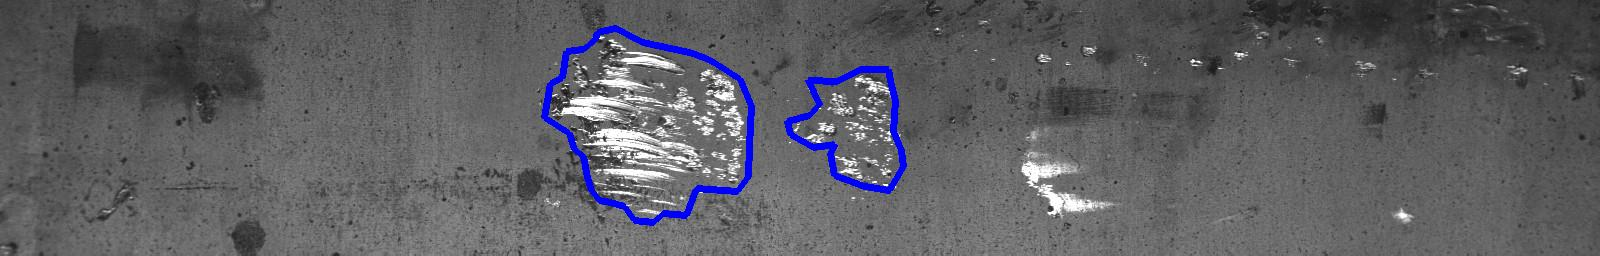
\includegraphics[width=\textwidth]{graphics/results/detector-result-class3-1}
	}
	\only<2-4> {
		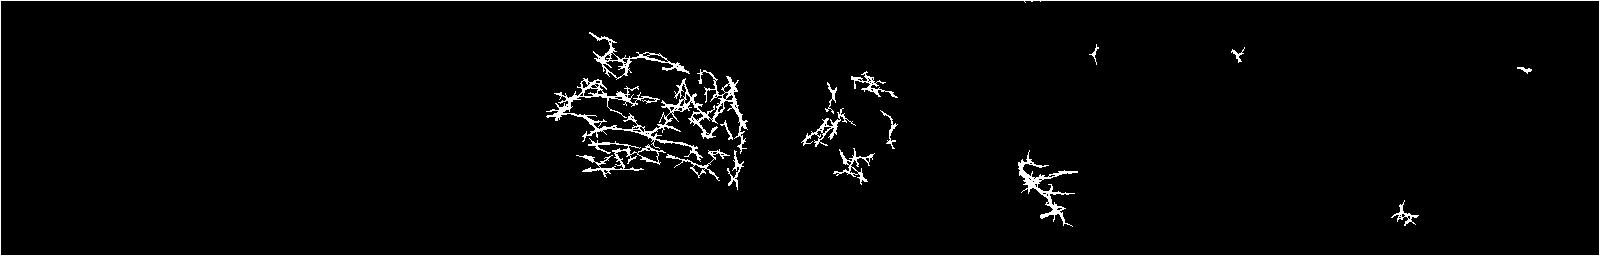
\includegraphics[width=\textwidth]{graphics/results/detector-result-class3-2}
	}
	\only<3-4> {
		
\includegraphics[width=\textwidth]{graphics/results/detector-result-class3-3}
	}
	\only<4> {
		
\includegraphics[width=\textwidth]{graphics/results/detector-result-class3-4}
	}
\end{frame}

\begin{frame}
\frametitle{Region proposals}
\framesubtitle{Example: Class No.4}
	\only<1-4> {
		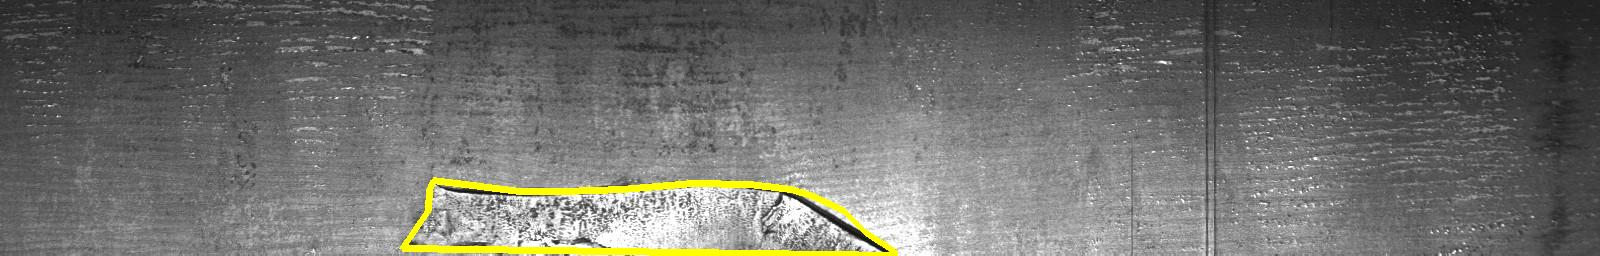
\includegraphics[width=\textwidth]{graphics/results/detector-result-class4-1}
	}
	\only<2-4> {
		
\includegraphics[width=\textwidth]{graphics/results/detector-result-class4-2}
	}
	\only<3-4> {
		
\includegraphics[width=\textwidth]{graphics/results/detector-result-class4-3}
	}
	\only<4> {
		
\includegraphics[width=\textwidth]{graphics/results/detector-result-class4-4}
	}
\end{frame}

\subsubsection{MC-CNN}
\begin{frame}{Multi Column CNN (MC-CNN)}
    \centering
    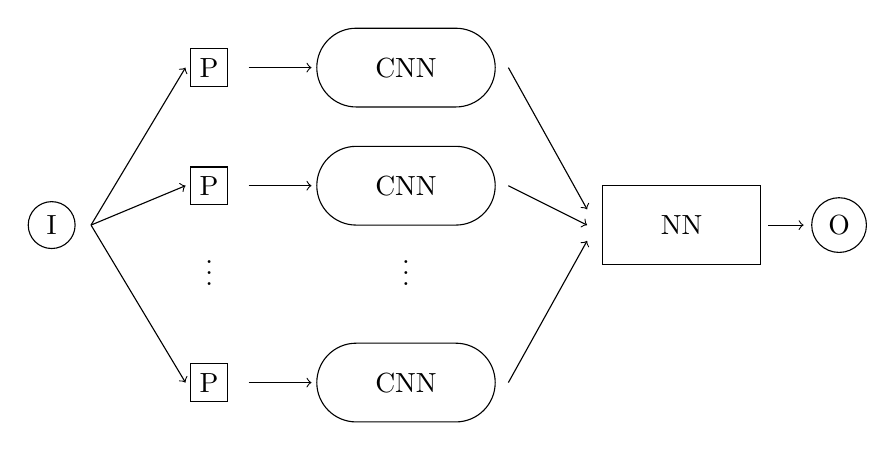
\begin{tikzpicture}
        % image
        \node[circle, draw] (input) at (0,0) {I};

        % preprocessed image
        \node[rectangle, draw] (p1) at ($(input) + (2,2)$) {P};
        \node[rectangle, draw] (p2) at ($(input) + (2,.5)$) {P};
        \node (p3) at ($(input) + (2,-.5)$) {\vdots};
        \node[rectangle, draw] (p4) at ($(input) + (2,-2)$) {P};

        % image to preprocessed image
        \draw[->] ($(input) + (0.5, 0)$) -- ($(p1) + (-0.3, 0)$);
        \draw[->] ($(input) + (0.5, 0)$) -- ($(p2) + (-0.3, 0)$);
        \draw[->] ($(input) + (0.5, 0)$) -- ($(p4) + (-0.3, 0)$);

        % cnn
        \node[rounded rectangle, draw, minimum width=2.5cm, minimum height=1cm] (cnn1) at ($(p1) + (2.5,0)$) {CNN};
        \node[rounded rectangle, draw, minimum width=2.5cm, minimum height=1cm] (cnn2) at ($(p2) + (2.5,0)$) {CNN};
        \node[minimum width=2.5cm, minimum height=1cm] (cnn3) at ($(p3) + (2.5,0)$) {\vdots};
        \node[rounded rectangle, draw, minimum width=2.5cm, minimum height=1cm] (cnn4) at ($(p4) + (2.5,0)$) {CNN};

        % preprocessed to cnn
        \draw[->] ($(p1) + (0.5, 0)$) -- ($(cnn1) + (-1.2, 0)$);
        \draw[->] ($(p2) + (0.5, 0)$) -- ($(cnn2) + (-1.2, 0)$);
        \draw[->] ($(p4) + (0.5, 0)$) -- ($(cnn4) + (-1.2, 0)$);

        % classifier
        \node[rectangle, draw, minimum width=2cm, minimum height=1cm] (classifier) at ($(cnn3) + (3.5,0.5)$) {NN};

        % cnn to classifier
        \draw[->] ($(cnn1) + (1.3, 0)$) -- ($(classifier) + (-1.2, .2)$);
        \draw[->] ($(cnn2) + (1.3, 0)$) -- ($(classifier) + (-1.2, 0)$);
        \draw[->] ($(cnn4) + (1.3, 0)$) -- ($(classifier) + (-1.2, -.2)$);

        % output
        \node[circle, draw] (output) at ($(classifier) + (2,0)$) {O};

        % classifier to output
        \draw[->] ($(classifier) + (1.1, 0)$) -- ($(output) + (-.45, 0)$);

    \end{tikzpicture}
\end{frame}

\begin{frame}{Multi Column CNN (MC-CNN)}
    \includegraphics[width=\textwidth]{graphics/architecture/mc-cnn-input}
    $$\Downarrow$$
    \centering
    \begin{tabular}{|c|c|c|c|c|}
        \hline
        Flawless area & Defect \#1 & Defect \#2 & Defect \#3 & Defect \#4\\\hline
        $1\%$ & $4\%$ & $6\%$ & \cellcolor{UniBlue}\textcolor{white}{$87\%$} & $2\%$ \\
        \hline
    \end{tabular}
\end{frame}

% \begin{frame}
%     \frametitle{Multi Column CNN (MC-CNN)}
%     \framesubtitle{Shape column}
%     \includegraphics[width=\textwidth]{graphics/architecture/mc-cnn-shape}
%     % \includegraphics[width=\textwidth]{graphics/architecture/mc-cnn-shape-architecture}
%     TODO confusion matrix + learning curve
% \end{frame}

% \begin{frame}
%     \frametitle{Multi Column CNN (MC-CNN)}
%     \framesubtitle{Local column}
%     \includegraphics[width=\textwidth]{graphics/architecture/mc-cnn-local}
%     % \includegraphics[width=\textwidth]{graphics/architecture/mc-cnn-shape-architecture}
%     TODO confusion matrix + learning curve
% \end{frame}

% \begin{frame}
%     \frametitle{Multi Column CNN (MC-CNN)}
%     \framesubtitle{Global column}
%     \includegraphics[width=\textwidth]{graphics/architecture/mc-cnn-global}
%     % \includegraphics[width=\textwidth]{graphics/architecture/mc-cnn-shape-architecture}
%     TODO confusion matrix + learning curve
% \end{frame}

\subsubsection{Output layer}
\begin{frame}{Output layer}
    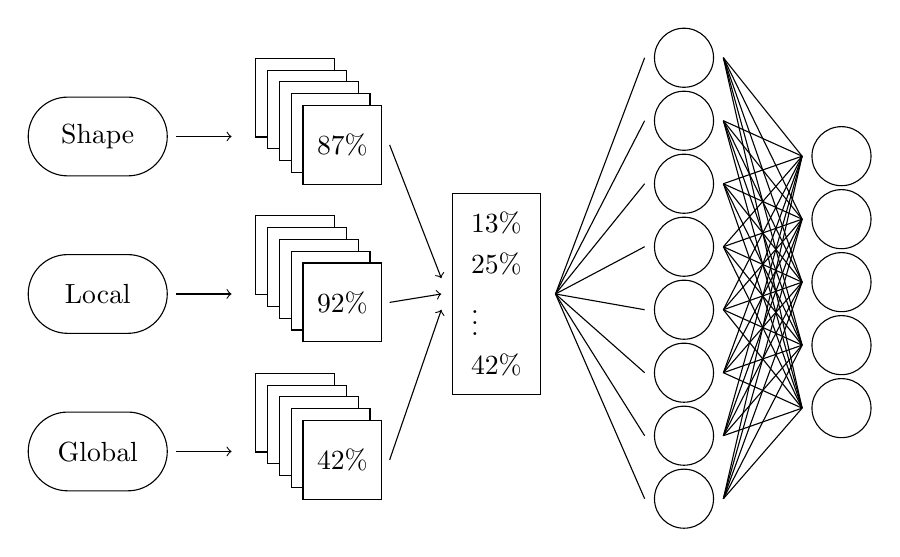
\begin{tikzpicture}

        % columns
        \node[rounded rectangle, draw, minimum width = 2cm, minimum height=1cm] (cnn1) at (0,2) {Shape};
        \node[rounded rectangle, draw, minimum width = 2cm, minimum height=1cm] (cnn2) at (0,0) {Local};
        \node[rounded rectangle, draw, minimum width = 2cm, minimum height=1cm] (cnn3) at (0,-2) {Global};

        % columns output
        \foreach \i in {0,...,4}
            \node[rectangle, draw, minimum width=1cm, minimum height=1cm, anchor=north west, fill=white] (output1 \i) at ($(cnn1) + (2+\i*0.15, 1-\i*.15) $) {$87\%$};

        \foreach \i in {0,...,4}
            \node[rectangle, draw, minimum width=1cm, minimum height=1cm, anchor=north west, fill=white] (output2 \i) at ($(cnn2) + (2+\i*0.15, 1-\i*.15) $) {$92\%$};

        \foreach \i in {0,...,4}
            \node[rectangle, draw, minimum width=1cm, minimum height=1cm, anchor=north west, fill=white] (output3 \i) at ($(cnn3) + (2+\i*0.15, 1-\i*.15) $) {$42\%$};

        % columns to output
        \draw[->] ($(cnn1) + (1, 0)$) -- ($(cnn1) + (1.7, 0)$);
        \draw[->] ($(cnn2) + (1, 0)$) -- ($(cnn2) + (1.7, 0)$);
        \draw[->] ($(cnn3) + (1, 0)$) -- ($(cnn3) + (1.7, 0)$);

        % fuse output
        \node [matrix, anchor=west, draw] (finalinput) at ($(cnn2) + (4.5,0)$)
        {
            \node {$13\%$};\\
            \node {$25\%$};\\
            \node {\vdots};\\
            \node {$42\%$};\\
        };

        % cnn output to flatten
        \draw[->] ($(output1 4) + (.6, 0)$) -- ($(finalinput) + (-.7,.2)$);
        \draw[->] ($(output2 4) + (.6, 0)$) -- ($(finalinput) + (-.7,0)$);
        \draw[->] ($(output3 4) + (.6, 0)$) -- ($(finalinput) + (-.7,-.2)$);

        % hidden layer
        \foreach \i in {0,...,7}
            \node[circle, draw, minimum width=.75cm, minimum height=.75cm, anchor=west] (h \i) at ($(finalinput) + (2, 3-\i*.8) $) {};
        \foreach \i in {0,...,7}
            \draw ($(finalinput) + (.75,0)$) -- ($(h \i) + (-.5,0)$);

        % output layer
        \foreach \i in {0,...,4}
            \node[circle, draw, minimum width=.75cm, minimum height=.75cm, anchor=west] (o \i) at ($(finalinput) + (4, 1.75-\i*.8) $) {};
        \foreach \i in {0,...,4}
            \foreach \j in {0,...,7}
                \draw ($(h \j) + (.5,0)$) -- ($(o \i) + (-.5,0)$);
        
        
    \end{tikzpicture}
    % FC NN + bayesopt params....
\end{frame}

\begin{frame}
    \frametitle{Multi Column CNN (MC-CNN)}
    \framesubtitle{Local column}
    \begin{columns}
        \column{.5\textwidth}
            Hello
%        \only<2> {
%            \column{.25}
%                % \includegraphics[height=\linewidth, angle=90, origin=c]{graphics/architecture/act_net}
%            \column{.25}
%                % \includegraphics[height=\linewidth, angle=90, origin=c]{graphics/architecture/act_net_hope}
%        }
    \end{columns}
\end{frame}


\subsection{Challenger}
\begin{frame}
    \frametitle{Challenger}
    \framesubtitle{Sliding window}
    \centering
    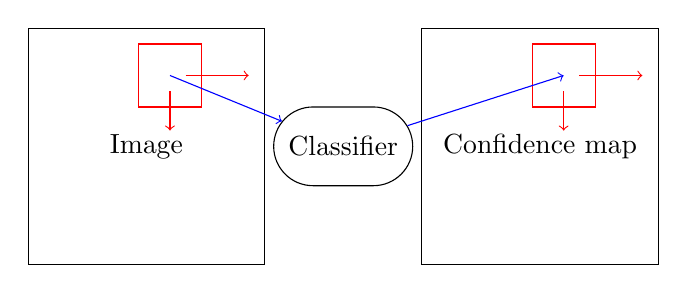
\begin{tikzpicture}
        % Image
        \node[rectangle, draw, minimum width=3cm, minimum height=3cm] (image) at (0,0) {Image};
        % Window
        \node[rectangle, draw=red, minimum width=.8cm, minimum height=.8cm] (window) at ($(image) + (.3,.9)$) {};
        % Sliding window
        \draw[->, draw=red] ($(window) + (.2,0)$) -- ($(window) + (1,0)$);
        \draw[->, draw=red] ($(window) + (0,-.2)$) -- ($(window) + (0,-.7)$);
        % Classifier
        \node[rounded rectangle, draw, minimum width=2cm, minimum height=1cm] (classifier) at ($(image) + (2.5,0)$) {Classifier};
        \draw[->,draw=blue] ($(window) + (0,0)$) -- (classifier);
        % Confidence map
        \node[rectangle,draw,minimum width=3cm, minimum height=3cm] (confidence map) at ($(classifier) + (2.5,0)$) {Confidence map};
        \node[rectangle, draw=red, minimum width=.8cm, minimum height=.8cm] (confidence map window) at ($(confidence map) + (.3,.9)$) {};
        \draw[->, draw=red] ($(confidence map window) + (.2,0)$) -- ($(confidence map window) + (1,0)$);
        \draw[->, draw=red] ($(confidence map window) + (0,-.2)$) -- ($(confidence map window) + (0,-.7)$);
        \draw[->,draw=blue] (classifier) -- ($(confidence map window)$);
    \end{tikzpicture}
\end{frame}

% \begin{frame}
%     \frametitle{Challenger}
%     \framesubtitle{Landmarks}
% \end{frame}
\section{Results}
    \begin{frame}{Results}
        \begin{center}
            \begin{tabular}{ |c|c|c|c|c|c|c| } 
             \hline
             Architecture & DCA [$\%$] & PCA [$\%$] & Overall Accuracy [$\%$]\\\hline
             Landmark & $90.24$ & $72.56$ & $80.94$\\ 
             Whatershed & $96.24$ & $82.56$ & $85.94$\\ 
             Proposed & $94.13$ & $93.16$ & $91.06$\\
             \hline
            \end{tabular}
            \vskip 1.5cm
            The project can be found in the \href{https://github.com/antonioterpin/wavelet_ml}{\texttt{GitHub repository}}
            \vskip 0.5cm
            \url{https://github.com/antonioterpin/wavelet_ml}
        \end{center}
    \end{frame}

% Extra slides
\section{Theoretical foundation (Extra)}
\subsection{Wavelet Analysis}
    \framepic{graphics/wavelets/wavelet}{
        \framefill
        \textcolor{black}{Wavelet}
        \vskip 0.5cm
    }

    \begin{frame}{Multi Resolution Analysis}
        \centering
        \onslide <1-> {
            \begin{block}{Goal}
                Approximate vectors of $L^2\left(\mathbb{R}\right)$ with variable degrees of resolution.
            \end{block}
        }
        \only <2> {
            \includegraphics[width=.6\textwidth]{graphics/wavelets/mra}
        }
        \only <3> {
            \includegraphics[width=.6\textwidth]{graphics/wavelets/mra-1}
        }
        \only <4> {
            \includegraphics[width=.6\textwidth]{graphics/wavelets/mra-2}
        }
        \only <5> {
            \includegraphics[width=.6\textwidth]{graphics/wavelets/mra-3}
        }
    \end{frame}

    \begin{frame}{Multi Resolution Analysis}
        \begin{block}{Axioms}
            \begin{equation}
                \cdots \subset V_{-2} \subset V_{-1} \subset V_0 \subset V_1 \subset V_2 \subset \cdots
            \end{equation}
            \begin{equation}
                \overline{\bigcup\limits_{n \in \mathbb{Z}} V_n} = L^2\left(\mathbb{R}\right)
            \end{equation}
            \begin{equation}
                \bigcap\limits_{n \in \mathbb{Z}} V_n = \left\{0\right\}
            \end{equation}
            \begin{equation}
                V_{n+1} = \mathcal{S}V_n
            \end{equation}
            \begin{equation}
                V_0 = \langle \left\{\tau^i\phi, i \in \mathbb{Z}\right\} \rangle \quad \exists \phi \in L^2\left(\mathbb{R}\right)\rangle
            \end{equation}
        \end{block}
    \end{frame}

    \begin{frame}{Multi Resolution Analysis}
        \begin{block}{Scaling function}
            \begin{equation}
                V_1 \supset V_0, \phi \in V_1
            \end{equation}
            \begin{equation}
                \left\{\mathcal{S}\tau^i\phi = \tau^{i/2}\mathcal{S}\phi, i \in \mathbb{Z}\right\} \; \text{orthonormal basis of } V_1
            \end{equation}
            \begin{equation}
                    \phi = \sum_{i \in \mathbb{Z}} g_i \tau^{i/2} \mathcal{S} \phi
            \end{equation}
        \end{block}
    \end{frame}

    \begin{frame}{Multi Resolution Analysis}
        \begin{block}{Wavelet}
            \begin{equation}
                V_{n+1} \supset V_n \Rightarrow \exists W_n \colon V_{n+1} = V_n \oplus W_n
            \end{equation}
            \begin{equation}
                \left\{\tau^i\psi\right\}_{i \in \mathbb{Z}} = W_0
            \end{equation}
            \begin{equation}
                \psi = \sum_{i \in \mathbb{Z}} h_i \tau^{i/2}\mathcal{S}\phi\quad\psi \in V_1
            \end{equation}
            \begin{equation}
                \langle \psi, \tau^i \psi \rangle = \delta_i
            \end{equation}
            \begin{equation}
                \langle \tau^j\psi, \tau^i \phi \rangle = 0
            \end{equation}
        \end{block}
    \end{frame}

    \begin{frame}
        \frametitle{Multi Resolution Analysis}
        \framesubtitle{Filter banks}
        \centering 
        \begin{tikzpicture}
            % High res
            \node[anchor= west] (highres) at (0,0) {$V_{n+1}$};
            % Low res
            \node[rectangle, draw, anchor= west, minimum height=0.75cm, minimum width=1.5cm] (g) at (3,2) {g};
            \node[circle, draw, anchor= west] (downsampleg) at (6,2) {$\downarrow 2$};
            \node[anchor= west] (lowres) at (8,2) {$V_n$};
            % Details
            \node[rectangle, draw, anchor= west, minimum height=0.75cm, minimum width=1.5cm] (h) at (3,-2) {h};
            \node[circle, draw, anchor= west] (downsampleh) at (6,-2) {$\downarrow 2$};
            \node[anchor= west] (details) at (8,-2) {$W_n$};

            \draw[->] (1,0) -- (2,0) -- (2,2) -- (3,2);
            \draw[->] (1,0) -- (2,0) -- (2,-2) -- (3,-2);

            \draw[->] (4.5,2) -- (6,2);
            \draw[->] (4.5,-2) -- (6,-2);

            \draw[->] (7,2) -- (8,2);
            \draw[->] (7,-2) -- (8,-2);

        \end{tikzpicture}
    \end{frame}

    \begin{frame}
        \frametitle{Wavelet: Example application}
        \framesubtitle{Detect abrupt changes}

        \centering
        \vskip -1cm
        $$s_1(t) = 2\sin\left(2\pi 10f_0 t\right) + \sin\left(2\pi 50f_0 t\right) + 10\delta\left(t - \frac{1}{2f_0}\right)$$
        \only<1> {
            \includegraphics[height=0.6\textheight]{graphics/wavelets/signal1}
        }
        \only<2> {
            \begin{columns}[onlytextwidth]
                \column{0.5\textwidth}
                \includegraphics[width=\textwidth]{graphics/wavelets/detect-abrupt-changes-fft}
                \column{0.5\textwidth}
                \includegraphics[width=\textwidth]{graphics/wavelets/detect-abrupt-changes-cwt}
            \end{columns}
        }

    \end{frame}

    \begin{frame}
        \frametitle{Wavelet: Example application}
        \framesubtitle{Detect temporal trends}
        $$f_{s_2} = e^t;\quad s_2 = \sin\left(2*pi*f_{s_2}t\right)$$
        \begin{columns}[onlytextwidth]
            \column{0.5\textwidth}
            \only<1-2> {
                \includegraphics[width=\textwidth]{graphics/wavelets/frequency-signal-2}
            }
            \only<3-4> {
                \includegraphics[width=\textwidth]{graphics/wavelets/detect-pattern-fft}
            }
            \column{0.5\textwidth}
            \only<2> {
                \includegraphics[width=\textwidth]{graphics/wavelets/signal2}
            }
            \only<4> {
                \includegraphics[width=\textwidth]{graphics/wavelets/detect-pattern-cwt}
            }
        \end{columns}
        
    \end{frame}


\subsection{Computer Vision}
    \framepic{graphics/computervision/computer-vision}{
        \framefill
        \textcolor{white}{Computer Vision}
        \vskip 0.5cm
    }
    \begin{frame}{Computer Vision}
        \begin{block}{Classification Task}
            To determine to which of a set of \textbf{categories} a given object belongs to.
        \end{block}
        \begin{columns}[onlytextwidth]
            \column{0.3\textwidth}
            \centering
            \includegraphics[width=\textwidth]{graphics/computervision/classification-image.jpeg}
            \onslide <2-> {
                \column{0.4\textwidth}
                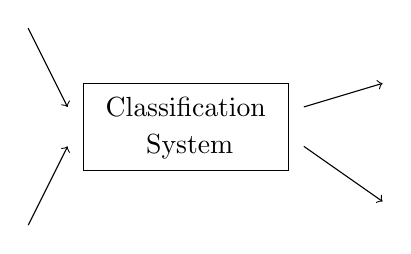
\begin{tikzpicture}
                    \node at (0,0) {Classification};
                    \node at (0.05,-0.5) {System};
                    \node[rectangle, draw, minimum width=2.6cm, minimum height=1.1cm, anchor=north west] at (-1.3,0.3) {};
                    \draw[->] (-2,1) -- (-1.5,0);
                    \draw[->] (-2,-1.5) -- (-1.5,-0.5);
                    \onslide <3-> {
                        \draw[->] (1.5,0) -- (2.5,0.3);
                        \draw[->] (1.5,-0.5) -- (2.5,-1.2);
                    }
                \end{tikzpicture}
            }
            \onslide <3-> {
                \column{0.2\textwidth}
                \vskip -0.5cm Output \vskip 0.5cm
                \begin{columns}[onlytextwidth]
                    \column{0.5\textwidth}
                        \begin{tabular}{|c|}
                            \hline
                            $0.03$\\\hline
                            \cellcolor{UniBlue}\textcolor{white}{$0.77$}\\\hline
                            $\vdots$\\\hline
                            $0.12$\\\hline
                        \end{tabular}
                    \column{0.5\textwidth}
                        \vskip -0.2cm
                        \begin{tabular}{c}
                            \\
                            \textcolor{UniBlue}{Child}\\
                            \\
                            \\
                        \end{tabular}
                \end{columns}
            }
        \end{columns}
    \end{frame}

    \begin{frame}{Computer Vision}
        \begin{block}{Object Localization Task}
            To find a given number (usually one) of items in a given context, predicting both their position and their class. \\
            \textbf{Remark.} Position is usually given as a bounding box.
        \end{block}
        \begin{columns}[onlytextwidth]
            \column{0.45\textwidth}
            \onslide <2-> {
                \includegraphics[width=\textwidth]{graphics/computervision/localization-input}
            }
            \column{0.45\textwidth}
            \onslide <3-> {
                \includegraphics[width=\textwidth]{graphics/computervision/localization-output}
            }
        \end{columns}
    \end{frame}

    \begin{frame}{Computer Vision}
        \onslide<1-> {
            \begin{block}{Object Detection Task}
                To \textbf{localize} any number of items in a given context, allowing either zero or any finite number of objects.
            \end{block}
        }
        \onslide<2-> {
            \begin{alertblock}{Remark.}
                The constraint on the number of object is \emph{a priori}. Indeed, a localization system will always look for a fixed number of objects, whereas a detection system is trained to be able to spot a variable number of objects in each input.
            \end{alertblock}
        }
    \end{frame}

    \begin{frame}{Computer Vision}
        \onslide <1-> {
            \begin{block}{Image Segmentation}
                Pixel-wide classification of the image. \textbf{Remark.} Image segmentation can be consider either the preemptive step to classification or the output of a classification system.
            \end{block}
        }
        \onslide <2-> {
            \vskip -0.5cm 
            \begin{exampleblock}{Example: Pixel-based image segmentation.}
                This family considers some distance defined over the image domain to segmentate it.
            \end{exampleblock}
        }
        \onslide <3-> {
            \vskip -0.5cm 
            \begin{exampleblock}{Example: Edge-based image segmentation.}
                This family uses an edge-detector algorithm, along with denoising and thresholding considerations, to solve the boundary detection problem.
            \end{exampleblock}
        }
    \end{frame}

    % \begin{frame}
    %     \frametitle{Pixel-based image segmentation}
    %     \framesubtitle{Whatershed}
    %     \begin{columns}[onlytextwidth]
    %         \column{0.5\textwidth}
    %         \includegraphics[width=\textwidth]{graphics/computervision/whatershed-plane}
    %         \column{0.5\textwidth}
    %         \includegraphics[width=\textwidth]{graphics/computervision/whatershed-surf}
    %     \end{columns}
    %     \only <1> {
    %         \begin{block}{Whatershed and immersion}
    %             The above pictures both show the same function defined over a 2D domain. Suppose to immerse the above right surface in some liquid, which gradually fill the two holes.
    %         \end{block}
    %     }
    %     \only <2> {
    %         \begin{block}{Whatershed and immersion}
    %             At some point the two volumes of liquid will meet, in particular they will flood at the same time over the green colored surface region.
    %         \end{block}
    %     }
    %     \only <3> {
    %         \begin{block}{Whatershed and immersion}
    %             This region is called whatershed and differentiates two areas of the image. Hence, an image can be segmentated considering its whatersheds.
    %         \end{block}
    %     }
    % \end{frame}

    % \begin{frame}
    %     \frametitle{Pixel-based image segmentation}
    %     \framesubtitle{Whatershed}
    %     % \includegraphics[width=\textwidth]{graphics/whatershed-plane}
    %     TODO insert example image\\
    %     % \includegraphics[width=\textwidth]{graphics/whatershed-surf}
    %     TODO insert example image
    % \end{frame}

    % \begin{frame}
    %     \frametitle{Pixel-based image segmentation}
    %     \framesubtitle{Whatershed}
    %     Let $\mathcal{D} \subset \mathbb{R}_+^2$ be a $2D$ domain, and $\mathcal{I} \colon \mathcal{D} \rightarrow \mathbb{R}_+$. Denote $\displaystyle h_m \triangleq \min_{\underline{x} \in \mathcal{D}}\mathcal{I}(\underline{x})$, $\displaystyle h_M \triangleq \max_{\underline{x} \in \mathcal{D}}\mathcal{I}(\underline{x})$, $T_h\left(\mathcal{I}\right) \triangleq \left\{\underline{p} \in \mathcal{D}, \mathcal{I}(\underline{p}) \leq h\right\}$.
    % \end{frame}

    % \begin{frame}
    %     \frametitle{Pixel-based image segmentation}
    %     \framesubtitle{Whatershed}
    %         \begin{itemize}
    %             \item Def, th, alg
    %             \item Example results
    %         \end{itemize}
    % \end{frame}

    \subsection{Image segmentation}
    \begin{frame}{$\alpha$-Shape}
        \onslide<1-> {
            \begin{alertblock}{Problem}
                The edge detector samples points along the boundary of the region. Moreover, this will always be an approximate sampling, because it is operating on a digital domain.
            \end{alertblock}
        }
        \onslide<2-> {
            \begin{exampleblock}{Solution}
                The $\alpha$-shape approach is a solution to a topologically correct image segmentation from a boundary sampling.
            \end{exampleblock}
        }
    \end{frame}
    \begin{frame}{$\alpha$-Shape}
        \onslide<1-> {
            \begin{definition}
                A \textit{partition} of the plane $\mathbb{R}^2$ is defined by a finite set of points $P = \left\{p_i\in\mathbb{R}^2\right\}$ and a set of pairwise disjoint arcs $A = \left\{a_i \subset \mathbb{R}^2\right\}$, such that $a_i\colon \left[0,1\right] \rightarrow \mathbb{R}^2;\; a_i(0), a_i(1) \in P$.
            \end{definition}
        }
        \onslide<2-> {
            \begin{definition}
                The union of the points and arcs is the \textit{boundary} of the partition $B = P \cup A$ and the regions $R = \left\{r_i \subset \mathbb{R}^2\right\}$ are the connected components of $B^C$.
            \end{definition}
        }
    \end{frame}
    \begin{frame}{$\alpha$-Shape}
        \onslide<1-> {
            \begin{definition}
                The partition is called \textit{binary} when:
                \begin{equation*}
                    \exists\;l\colon R \rightarrow \left\{0,1\right\} \text{ s.t. }\forall r_i \neq r_j \in R\; \overline{r_i} \cap \overline{r_j} = \emptyset \lor l\left(r_i\right) \neq l\left(r_j\right)
                \end{equation*}
            \end{definition}
        }
        \begin{columns}
            \column{.5\linewidth}
                \onslide<2-> {
                    \begin{definition}
                        A plane partition is \textit{$r$-stable} when its boundary can be dilated with a closed disc of radius $s$ without changing its homotopy type for any $s \leq r$.
                    \end{definition}
                }
            \column{.4\linewidth}
                \onslide<3-> {
                    \includegraphics[width=\linewidth]{graphics/theory-extra/rstable}
                }
        \end{columns}
    \end{frame}
    \begin{frame}{$\alpha$-Shape}
        \onslide<1-> {
            \begin{definition}
                A finite set of sampling points $\mathcal{S} = \left\{s_i \in \mathbb{R}^2\right\}$ is called a $\left(p, q\right)$-sampling of the boundary $B$ when: 
                \begin{itemize}
                    \item $\forall b \in B, \max\left\{\min\left\{d\left(b,s\right),\; s \in \mathcal{S}\right\}\right\} \leq p$
                    \item $\forall s \in \mathcal{S}, \max\left\{\min\left\{d\left(b,s\right),\; b \in B\right\}\right\} \leq q$
                \end{itemize} 
                For some $d(\cdot,\cdot)$. The elements of $\mathcal{S}$ are called \textit{edgels}. The sampling is said to be \textit{strict} when all edgels are exactly on the boundary, i.e. $q = 0$.
            \end{definition}
        }
        \onslide<2-> {
            \vskip -1cm
            \begin{columns}
                \column{.5\textwidth}
                \centering
                \begin{tikzpicture}[rotate=-50]
                    % \draw[step=.5cm,gray,very thin] (0,0) grid (4,4);
                    \draw (0,0) .. controls (0,4) and (4,0) .. (4,4);
                    \foreach \Point in {(.1,.4), (0,1), (.3,1.3), (1,2), (1.5,2), (2.1,1.9), (2.35,2.1), (3,2.1), (3.5,2.5), (3.75,2.4), (3.75,3), (4, 3.75)}{
                        \node[color=ForestGreen] at \Point {\textbullet};
                    }
                    \foreach \Point in {(.25,2.25), (1,1.5), (1.5,2.5), (2.5,2.5), (3,1.5), (3.5,3)}{
                        \node[color=Red] at \Point {$\star$};
                    }
                \end{tikzpicture}
                \column{.5\textwidth}
                \vskip -.5cm
                \begin{itemize}
                    \item $\forall b \in B \;\exists$ \textcolor{ForestGreen}{\textbullet} such that $d(b, \text{\textcolor{ForestGreen}{\textbullet}}) \leq p$.
                    \item $\forall s = \text{\textcolor{ForestGreen}{\textbullet}}, \text{\textcolor{Red}{$\star$}} \;\exists b \in B$ such that $d(b,s) \leq q$.
                \end{itemize}
            \end{columns}
        }
    \end{frame}
    \begin{frame}{$\alpha$-Shape}
        \onslide<1-> {
            \vskip -.5cm
            \begin{definition}
                The \textit{Delaunay triangulation} $\mathcal{D}$ of a set of point $\mathcal{S}$ is the subset of all triangles $T = \left\{\left(a, b, c\right) \subset \mathcal{S}^3, a \neq b, b \neq c, a \neq c \right\}$ such that $t \in T, x \in \mathcal{S} \Rightarrow x \not\in \mathcal{C}\left(t\right)$, where $\mathcal{C}\left(t\right)$ is the circumcircle of $t$.
            \end{definition}
        }
        \onslide<2-> {
            \vskip -.25cm
            \begin{definition}
                The union of cells $c \in \mathcal{D}$ is called \textit{polytope} of $\mathcal{D}$. 
                \begin{equation*}
                    \mathcal{D}_\alpha = \left\{t \in T \colon r\left(\mathcal{C}\left(t\right)\right) < \alpha\right\},
                \end{equation*}
                where $r\left(\mathcal{C}\left(t\right)\right)$ is the radius of the circumcircle of $t$. The polytope of $\mathcal{D}_\alpha$ is called \textit{alpha-shape}.
            \end{definition}
        }
        \onslide<3-> {
            \vskip -.75cm
            \begin{remark}
                $\alpha$ is the first Bayesian optimization parameter regarding the $\alpha$-shape.
            \end{remark}
        }
    \end{frame}
    \begin{frame}{$\alpha$-Shape}
        \begin{columns}[onlytextwidth]
            \column{0.5\textwidth}
                \onslide <1-> {
                    \includegraphics[width=\textwidth]{graphics/computervision/detector-points}
                }
                \vskip -.7cm
                \onslide <4-> {
                    \includegraphics[width=\textwidth]{graphics/computervision/detector-convhull}
                }
            \column{0.5\textwidth}
                \onslide <2-> {
                    \includegraphics[width=\textwidth]{graphics/computervision/detector-a-shape}   
                }
                \vskip -.7cm
                \onslide <3-> {
                    \includegraphics[width=\textwidth]{graphics/computervision/detector-a-shape-better-radius}
                }
            
        \end{columns}
    \end{frame}
    \begin{frame}{$\alpha$-Shape}
        \onslide<1-> {
            \begin{lemma}
                The union of closed $\alpha$-discs with centers at the points $s_i \in \mathcal{S}$ covers $\lvert \mathcal{D}_\alpha \rvert$, and the two sets are homotopy equivalent.\newline
                % \textbf{Proof.} (Blackboard)
            \end{lemma}
        }
        \onslide<2-> {
            What are then the conditions of homotopy equivalence between the boundary and the alpha shape?
        }
        \onslide<3-> {
            \includegraphics[width=\linewidth]{graphics/theory-extra/topologicalequivalence-border-ashape}
        }
    \end{frame}

    \begin{frame}{$\alpha$-Shape}
        \onslide<1-> {
            \begin{definition}
                A connected component of $\lvert\mathcal{D}_\alpha\rvert^C = \mathbb{R}^2 \setminus \lvert \mathcal{D}_\alpha \rvert$ is called an $\alpha$-hole of $\lvert\mathcal{D}_\alpha\rvert$. When the radius of the circumcircle of the largest Delaunay triangle in an $\alpha$-hole’s closure is at least $\beta \geq \alpha$, we speak of an $\left(\alpha, \beta\right)$-hole.
            \end{definition}
        }
        \onslide<2-> {
            \begin{lemma}
                An $\alpha$-hole $h$ is an $\left(\alpha,\beta\right)$-hole if and only if it contains a point $v$ whose distance from the nearest edgel is at least $\beta$.\newline
                % \textbf{Proof.} (Blackboard)
            \end{lemma}
        }
    \end{frame}

    \begin{frame}{$\alpha$-Shape}
        \onslide<1-> {
            \begin{definition}
                An $\left(\alpha,\beta\right)$-boundary reconstruction from an edgel set $\mathcal{S}$ is defined as the union of the polytope $\lvert\mathcal{D}_\alpha\rvert$ with all $\alpha$-holes of $\mathcal{D}_\alpha$ that are not $\left(\alpha,\beta\right)$-holes.
            \end{definition}
        }
        \onslide<2-> {
            \begin{remark}
                Therefore, $\beta$ is related to the \textit{hole-threshold} Bayesian optimization parameter.
            \end{remark}
        }
    \end{frame}

    \begin{frame}{$\alpha$-Shape}
        \begin{theorem}
            Let $P$ be an $r$-stable plane partition, and $S$ a $\left(p,q\right)$-sampling of $P$’s boundary $B$. Then the $\left(\alpha,\beta\right)$-boundary reconstruction $R$ defined by $S$ is homotopy equivalent to $B$, and the $\left(\alpha,\beta\right)$-holes of $R$ are topologically equivalent to the regions $r_i$ of $P$, if:
            \begin{itemize}
                \item $p < \alpha \leq r - q$
                \item $\beta = \alpha + p + q$
                \item $\forall r_i \in R \;\exists \gamma \geq \beta + q > 2\left(p+q\right)$ such that $r_i$ contains an open $\gamma$-disc.
            \end{itemize}
            % \textbf{Proof.} (Blackboard)
        \end{theorem}
    \end{frame}
\subsection{Optimization}
\begin{frame}
    \frametitle{Optimization}
    \onslide <1-> {
        \begin{block}{Bayesian optimization}
            Bayesian optimization aims to solve an optimization problem $\max\limits_{x\in A}f\left(x\right)$ when:
            \begin{itemize}
                \item $A \subset \mathbb{R}^d$ with $d$ not too large.
                \item Easy to asses $A$ membership.
                \item $f$ can be modeled using \emph{Gaussian process regression}.
                \item $f$ is a \emph{black box}.
            \end{itemize}
        \end{block}
    }
    \onslide <2-> {
        \begin{exampleblock}{Loss function}
            \begin{equation}
                J\left(\alpha\right) = \frac{2\lvert X \cap Y \rvert}{\lvert X \rvert + \lvert Y \rvert} = -f(x)
            \end{equation}
        \end{exampleblock}
    }
\end{frame}

\begin{frame}
    \frametitle{Optimization}
    \vskip -0.5cm
    \begin{block}{Bayesian optimization}
        Firstly a collection of points $x_1, \ldots, x_k \in \mathbb{R}^d$ is considered. Suppose $f$ can be modeled as:
        \begin{equation*}
            f\left(x_{1:n}\right) \sim \mathcal{N}\left(\mu\left(x_{1:n}\right), \Sigma\left(x_{1:n}, x_{1:n}\right)\right)
        \end{equation*}
        Then we can infere the probability distribution of $f\left(x_{n+1}\right)$:
        \begin{equation}
            f\left(x_{n+1}\right) \mid f\left(x_{1:n}\right) \sim \mathcal{N}\left(\mu_{n+1}, \Sigma_{n+1}\right)
        \end{equation}
        \begin{equation*}
            \mu_{n+1} = \Sigma\left(x_{n+1}, x_{1:n}\right)\Sigma\left(x_{1:n}, x_{1:n}\right)^{-1}\left(f\left(x_{1:n}\right) - \mu\left(x_{1:n}\right)\right) + \mu\left(x_{n}\right)
        \end{equation*}
        \begin{equation*}
            \Sigma_n = \Sigma\left(x_{n+1}, x_{n+1}\right) - \Sigma\left(x_{n+1}, x_{1:n}\right)\Sigma\left(x_{1:n}, x_{1:n}\right)^{-1}\Sigma\left(x_{1:n}, x_{n+1}\right)
        \end{equation*}
    \end{block}
\end{frame}

\begin{frame}
    \frametitle{Optimization}
    \begin{exampleblock}{Acquisition function}
        Therefore, it is possible to consider an \emph{acquisition function}, i.e. a function that given the previous $x_1, \ldots, x_n$ values determines the best choice of $x_{n+1}$:
        \begin{equation}
            a \colon \left[x_1 \ldots x_n\right] \rightarrow x_{n+1} \colon \mathcal{P}\left[f(x_{n+1}) = \max\limits_{x \in A} f\left(x\right)\right] \text{is max}
        \end{equation}
    \end{exampleblock}
\end{frame}
\subsection{Deep Learning}
    \framepic{graphics/deeplearning/deep-learning}{
        \framefill
        \textcolor{white}{Deep Learning}
        \vskip 0.5cm
    }

    \begin{frame}{Computer Vision}
        \begin{block}{Classification Task}
            To determine to which of a set of \textbf{categories} a given object belongs to.
        \end{block}
        \begin{columns}[onlytextwidth]
            \column{0.3\textwidth}
            \centering
            \includegraphics[width=\textwidth]{graphics/computervision/classification-image.jpeg}
            \onslide <2-> {
                \column{0.4\textwidth}
                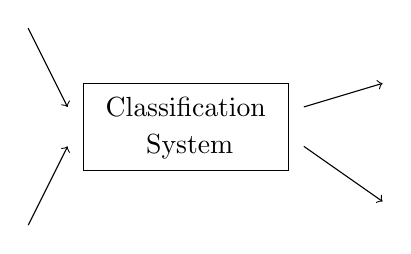
\begin{tikzpicture}
                    \node at (0,0) {Classification};
                    \node at (0.05,-0.5) {System};
                    \node[rectangle, draw, minimum width=2.6cm, minimum height=1.1cm, anchor=north west] at (-1.3,0.3) {};
                    \draw[->] (-2,1) -- (-1.5,0);
                    \draw[->] (-2,-1.5) -- (-1.5,-0.5);
                    \onslide <3-> {
                        \draw[->] (1.5,0) -- (2.5,0.3);
                        \draw[->] (1.5,-0.5) -- (2.5,-1.2);
                    }
                \end{tikzpicture}
            }
            \onslide <3-> {
                \column{0.2\textwidth}
                \vskip -0.5cm Output \vskip 0.5cm
                \begin{columns}[onlytextwidth]
                    \column{0.5\textwidth}
                        \begin{tabular}{|c|}
                            \hline
                            $0.03$\\\hline
                            \cellcolor{UniBlue}\textcolor{white}{$0.77$}\\\hline
                            $\vdots$\\\hline
                            $0.12$\\\hline
                        \end{tabular}
                    \column{0.5\textwidth}
                        \vskip -0.2cm
                        \begin{tabular}{c}
                            \\
                            \textcolor{UniBlue}{Child}\\
                            \\
                            \\
                        \end{tabular}
                \end{columns}
            }
        \end{columns}
    \end{frame}

    \begin{frame}{Computer Vision}
        \begin{block}{Object Localization Task}
            To find a given number (usually one) of items in a given context, predicting both their position and their class. \\
            \textbf{Remark.} Position is usually given as a bounding box.
        \end{block}
        \begin{columns}[onlytextwidth]
            \column{0.45\textwidth}
            \onslide <2-> {
                \includegraphics[width=\textwidth]{graphics/computervision/localization-input}
            }
            \column{0.45\textwidth}
            \onslide <3-> {
                \includegraphics[width=\textwidth]{graphics/computervision/localization-output}
            }
        \end{columns}
    \end{frame}

    \begin{frame}{Computer Vision}
        \onslide<1-> {
            \begin{block}{Object Detection Task}
                To \textbf{localize} any number of items in a given context, allowing either zero or any finite number of objects.
            \end{block}
        }
        \onslide<2-> {
            \begin{alertblock}{Remark.}
                The constraint on the number of object is \emph{a priori}. Indeed, a localization system will always look for a fixed number of objects, whereas a detection system is trained to be able to spot a variable number of objects in each input.
            \end{alertblock}
        }
    \end{frame}

    \begin{frame}{Computer Vision}
        \onslide <1-> {
            \begin{block}{Image Segmentation}
                Pixel-wide classification of the image. \textbf{Remark.} Image segmentation can be consider either the preemptive step to classification or the output of a classification system.
            \end{block}
        }
        \onslide <2-> {
            \vskip -0.5cm 
            \begin{exampleblock}{Example: Pixel-based image segmentation.}
                This family considers some distance defined over the image domain to segmentate it.
            \end{exampleblock}
        }
        \onslide <3-> {
            \vskip -0.5cm 
            \begin{exampleblock}{Example: Edge-based image segmentation.}
                This family uses an edge-detector algorithm, along with denoising and thresholding considerations, to solve the boundary detection problem.
            \end{exampleblock}
        }
    \end{frame}

    \begin{frame}{Training}
        \begin{block}{Forward propagation}
            The \emph{feedforward} neural network accepts an input $\underline{\underline{X}}$ and produce an output $\underline{y}$. The information from $\underline{\underline{X}}$ flows through the hidden units to produce $\underline{y}$. This is called \textbf{forward propagation}.
        \end{block}

        \begin{block}{Backward propagation}
            During the training the forward propagation can continue onward to evaluate a scalar cost $J\left(\underline{\underline{\theta}}\right)$. The \textbf{back-propagation} algorithm is a numerically efficient way to compute cost gradient, in order to perform gradient descent.
        \end{block}    
    \end{frame}

    \begin{frame}{Deep Learning}
        \includegraphics[width=\textwidth]{graphics/deeplearning/nn}
    \end{frame}

    \begin{frame}
        \frametitle{Training}
        \framesubtitle{Backpropagation (proof)}
        \centering
        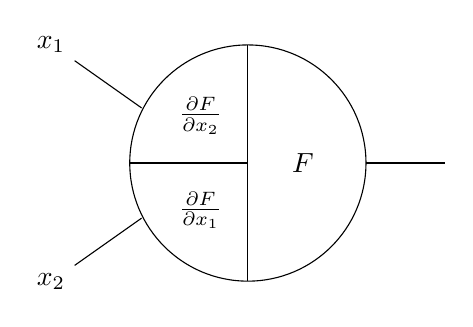
\begin{tikzpicture}
            \node[circle, draw, minimum width=3cm, minimum height=3cm] at (0,0) {};
            \node at (0.7,0) {$F$};
            \node at (-0.6,-0.6) {$\frac{\partial F}{\partial x_1}$};
            \node at (-0.6,0.6) {$\frac{\partial F}{\partial x_2}$};
            \node at (-2.5,1.5) {$x_1$};
            \node at (-2.5,-1.5) {$x_2$};

            \draw (0,0) -- (-1.5,0);
            \draw (0,-1.5) -- (0,1.5);
            \draw (1.5, 0) -- (2.5,0);

            \draw (-1.35, 0.7) -- (-2.2,1.3);
            \draw (-1.35, -0.7) -- (-2.2,-1.3);
        \end{tikzpicture}

        \vskip 0.5cm
        
        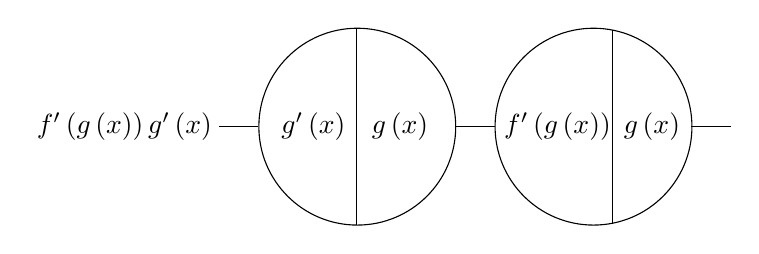
\begin{tikzpicture}
            \node at (-.7,0) {$f'\left(g\left(x\right)\right)g'\left(x\right)$};

            \draw (0.5,0) -- (1,0);

            \node[circle, draw, minimum width=2.5cm, minimum height=2.5cm, anchor=west] at (1,0) {};
            \node at (1.7, 0) {$g'\left(x\right)$};
            \node at (2.8, 0) {$g\left(x\right)$};
            \draw (2.25, 1.25) -- (2.25, -1.25);

            \draw (3.5, 0) -- (4, 0);

            \node[circle, draw, minimum width=2.5cm, minimum height=2.5cm, anchor=west] at (4,0) {};
            \node at (4.8, 0) {$f'\left(g\left(x\right)\right)$};
            \node at (6, 0) {$g\left(x\right)$};
            \draw (5.5, 1.23) -- (5.5, -1.23);

            \draw (6.5, 0) -- (7, 0);

        \end{tikzpicture}
    \end{frame}

    \begin{frame}{Convolutional Networks}
        \includegraphics[width=\textwidth]{graphics/deeplearning/cnn}
        \vskip 0.5cm
        \begin{exampleblock}{Motivation}
            \begin{enumerate}
                \item Sparse interactions
                \item Parameter sharing
                \item Equivariant representations
                \item Biologically inspired artificial intelligence
            \end{enumerate}
        \end{exampleblock}
    \end{frame}

    \begin{frame}{Convolutional Networks}
        \includegraphics[width=\textwidth]{graphics/deeplearning/cnn}
        \onslide <1-> {
            \begin{block}{Convolutional neural networks (CNN)}
                CNNs are a specialized kind of neural network for processing data that has a known grid-like topology.
            \end{block}
        }
        \onslide <2-> {
            \begin{block}{Convolutional neural networks (CNN) - 2}
                CNNs are neural networks that use convolution in place of general matrix multiplication in at least one of their layers.
            \end{block}
        }
    \end{frame}

% \begin{frame}[t,allowframebreaks]
% \frametitle{Bibliography}

% \nocite{*} % will display the non-cited publications as well. Useful for a publication list.

% \printbibliography

% \end{frame}

\end{document}